\section{Building robots}


As work on the perception side commenced, the question how an agent using such a filter system would behave in a real-world scenario became apparent.
This would allow to study behavioral patterns in more details, benchmark, and enhance quality of the algorithms.
The robot's platform should hold the following constraints:

\begin{itemize}
  \item the central computing board should be the same for all robots and powerful enough to perform computer vision tasks,
  \item the same code base should be used for all robots; hardware specific specialization should be off-loaded into separate code classes,
  \item sensors should be connectable via modern bus systems as \wire\ and \ic,
  \item the framework should generalize well and be easily extensible, and
  \item all robots should be able to communicate to each other via a central \gls{ac:wlan} node or peer-to-peer via Bluetooth.
\end{itemize}

It was decided to use a Raspberry Pi mini computer as computing platform.
Currently, it offers a quad-core \gls{ac:cpu} with \unit[1.4]{GHz}, a memory of \unit[1]{GB} and an onboard Bluetooth and \gls{ac:wlan} chip.
Additionally, an \gls{ac:imu} is attached to all robots, measuring lateral and rotational acceleration.
The robots are shown in \figref{fig:robot_introduction_photo}.
In total, there were two wheeled robots (\figref{fig:robot_introduction_photo_wheelpi}) and one flying robot, \figref{fig:robot_introduction_photo_flypi}, using a quadrotor design, built.

\begin{figure}
  \centering
  \begin{subfigure}[]{0.475\textwidth}
    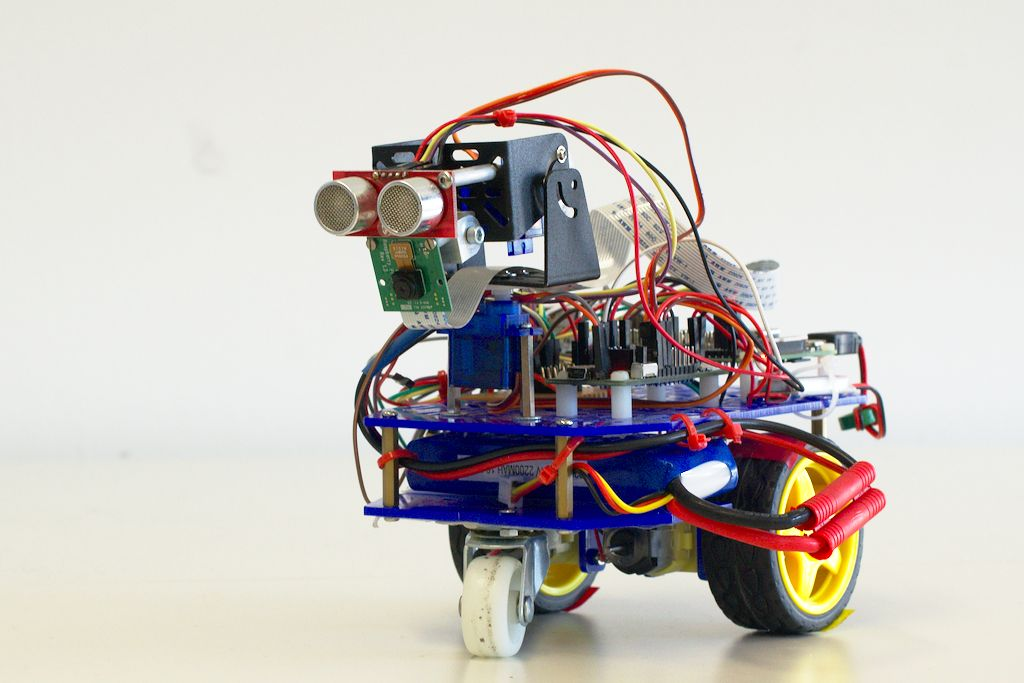
\includegraphics[width=1.0\textwidth]{./figures/robot/photos/wheelpi.jpg}
    \caption{WheelPi robot.}
    \label{fig:robot_introduction_photo_wheelpi}
  \end{subfigure}
  \hfill
  \begin{subfigure}[]{0.475\textwidth}
    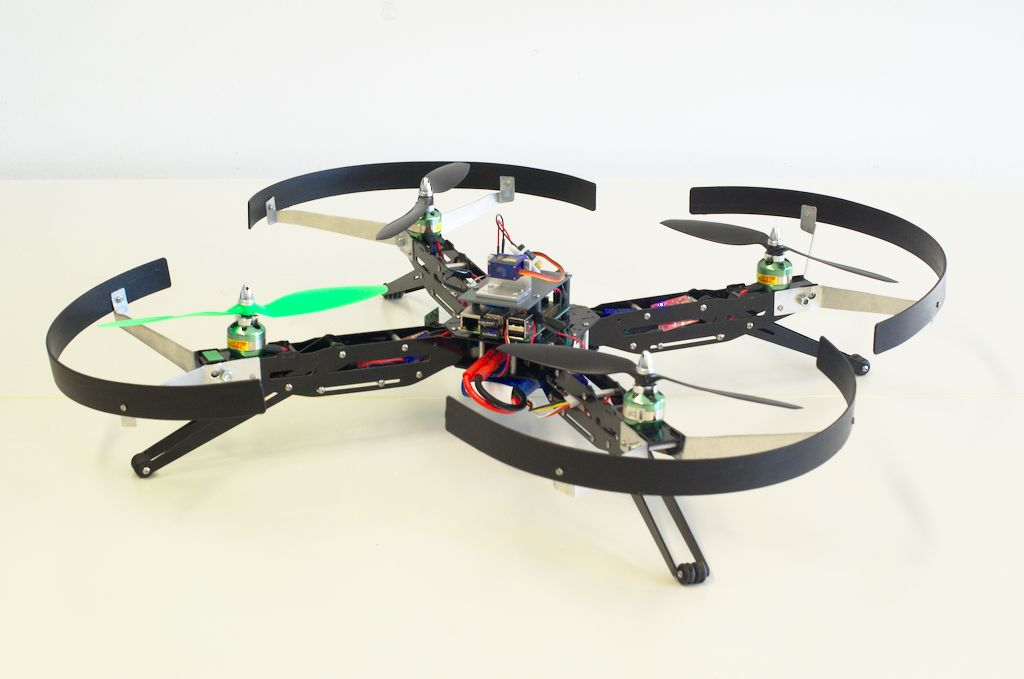
\includegraphics[width=1.0\textwidth]{./figures/robot/photos/quadcopter.jpg}
    \caption{FlyPi robot.}
    \label{fig:robot_introduction_photo_flypi}
  \end{subfigure}
  \caption{The pictures show the robots used in this work. On the left, there is the WheelPi robot: a three-wheeled ground-based robot. In \figref{fig:robot_introduction_photo_flypi} the FlyPi robot is shown. It is a flying robot utilizing a quadrotor design. Both robots are part of the MovingPi library.}
  \label{fig:robot_introduction_photo}
\end{figure}

Given the constraints from above, the objective of this project is:

\begin{enumerate}
  \item Develop a framework, which can be easily deployed on different hardware designs,
  \item Utilize the framework on multiple agents,
  \item Each agent localizes itself in a previously unknown environment,
  \item Information about the environment, \ie maps are shared across all agents.
\end{enumerate}

Parts of the here presented work is published in~\textcite{reichseerberscheid2018} and numerous students have contributed to this elaborate project.
They are listed above at the beginning of this thesis.





\section{Introduction}
\label{sec:robot_introduction}

Humans may easily navigate inside a room.
We have stereo vision, allowing for 3d vision\footnote{At least most of us.}.
We can segment our visual field into subsets, where each subset represents a meaningful entity, \eg. an object.
Because we are able to perform all this intuitively, this is a deceptively tricky business.
One of the pioneers of \gls{ac:ai}, Marvin Minsky, invited to a summer school in 1966 called ``The Summer Vision Project''.
A Memo written by one of his research associates, Seymour Papert, outlines the project goals~\cite[p. 2f]{papert1966summer}:

\begin{enumerate}
  \item ``The primary goal\ldots\ is to\ldots\ divide a\ldots\ picture into regions such as
    \begin{itemize}
      \item likely objects
      \item likely background areas
      \item chaos.''
    \end{itemize}
  \item ``considerable analysis of shape and surface properties'' and ``region description''.
  \item ``The final goal is object identification which will actually name objects by matching them with a vocabulary of known objects.''
\end{enumerate}

Nearly half a century later, \acrlong{ac:dnn} have shown promising results towards these goals~\cite{krizhevsky2012imagenet, deng2009imagenet, kim2014convolutional}.
Despite these extensive efforts to solve the ``construction of a significant part of a visual system''~\cite[p. 1]{papert1966summer}, a long road to complete ``computer vision'' remains.
In fact, this is just another form of Moravec's Paradox shown in \secref{ssec:introduction_motivation}; Tasks, which are easy for human being are computational expensive for machines.

In this work, the focus lies on fully autonomous robots.
All computations must be performed on embedded hardware, \ie utilizing only limited computational power, and must run online in real-time.
Especially the flying robot, \figref{fig:robot_introduction_photo_flypi}, also named \gls{ac:aav}, must at all times provide safe error propagation and fallback settings.
On embedded hardware, without the support of large multi-core \glspl{ac:cpu} or \glspl{ac:gpu}, robots usually perform with a low frame rate.
One of the most challenging applications is visual guided on-board-computed indoor flight.
There are no \gls{ac:gps} signals available and the autonomous vehicle has to navigate quickly in confined spaces.
To enable collision detection, onboard sensors have to be utilized.
Truly autonomous robots --- without mandatory connection to a stationary computing system --- and without the need of external sensors for navigation, may be used for example in indoor search-and-rescue missions, disaster relief in dangerous environments (as for example it was the case in Fukushima, Japan, 2011~\cite{chino2011preliminary}), reconnaissance, or underground mining operations.

In recent years, energy efficient, yet powerful hardware and batteries have become available.
Moreover, the hardware physical dimensions have been reduced a lot.
This allows on one hand for smaller robots and on the other hand for complex online motor control tasks and sensor evaluation --- as it is required in quadrocopters.
However, active sensor approaches pose the problem of high power consumption and heavy weight.
On today's robots these problems are solved by using an RGB camera.
RGB cameras are passive sensors with low power consumption.

Previous work on autonomous flight can be categorized into two research areas.
First, many works focus on agile and accurate motion control. Most prominent is the quadrocopter swarm of ETH Zurich, which is able to perform synchronized dancing motions~\cite{schSPRI14}, build simple architectural structures~\cite{augugliaro2014flight}, or even knot strings and build a bridge~\cite{augugliaro2015knot}. 
But these complex tasks heavily rely on external tracking of the robots and are thus restricted to lab use~\cite{brescianini2018trajectory}. 
In another approach, artificial markers in the environment simplify pose estimation~\cite{eberli2011vision}. 
For \gls{ac:gps} enabled areas, complete commercial solutions exist, \eg~\cite{vasarhelyi2014outdoor,radiansyah2017quadcopter}.

Second, there are approaches, which only use online sensors for self localization.
Still, in many studies the computationally expensive tasks are performed on external hardware via Bluetooth or \gls{ac:wlan} links, \eg~\cite{engel14ras,zhang2016controllable}, which limit the independence of the devices.
In recent years, the miniaturization of computers and advancements in battery design, driven mostly by rapid cell phone development, have made it possible to build smaller autonomous robots and perform computations in real-time on the \gls{ac:aav} itself.
While online computations result in maximum autonomy, even today, real-time computations on 3d data remain too complex a task.
Instead of 3d sensors such as LIDAR, the Asus Xtion Pro, or the Microsoft Kinect sensor, most systems use a monocular camera and perform 3d reconstruction.

For example, the detection of a planar landing zone for a helicopter using a monocular camera is described in~\cite{5584396} in 2010, allowing for autonomous landing of a helicopter.
Following up on this work, seven years later similar results are shown for a moving platform~\cite{falanga2017vision}.
Here, the robot relies only on its internal sensors and lands autonomously on a platform, which holds a marker and moves in a straight line with up to $\unit[4.2]{m/s}$.
\cite{6630807} use a front facing camera to detect objects in the flight path and estimate size.
In recent studies more stable SLAM methods were introduced, \eg~\cite{7219438,engel2014lsd,engel2017direct}, which promise good results for front-facing cameras.
However, these methods are computationally too expensive for embedded hardware.
Also, all approaches with a camera pointing to a specific direction face the problem of a small observation window with significant feature shifts in consecutive camera frames.

Omnidirectional monocular cameras, which provide a 360$\degree$ view of the environment, have been successfully applied to these problems.
Already in 2006 in~\cite{demonceaux2006omnidirectional} full attitude measurements were reported.
\cite{rodriguez2012real} apply this procedure to an unstable flying robot; however, no quantitative results are shown.
In~\cite{lukierski2017room}, a fast moving robot estimates the depth of edges in a corridor using an omnidirectional camera.
In~\cite{forster2014svo} a visual odometry algorithm is introduced, which tracks features and computes frame based pose displacement.
The authors report a frame rate of $\unit[55 \pm 1]{Hz}$, but computations are only performed on certain key frames.

In this work, the focus lies on navigating a flying robot in unknown, GPS-denied, indoor scenarios.
All computations are performed online and in real-time --- there will be no external tracking.
We ask: what is needed to safely (and therefore reliably) detect features on a hardware platform that strongly jerks, jolts, and may even flip?
And --- if those can be found --- how to track them and use them for trajectory planning on limited hardware in real-time?
One goal is to improve navigation by introducing a novel lightweight omnidirectional camera setup for embedded computer systems.
Lastly, the aim is to extract features, track them over multiple frames, compute a 3d point cloud, and perform high level navigation tasks on this internal model of the \gls{ac:aav}'s environment.

In the following section, we shortly introduce our hardware approach, a quadrocopter holding an omnidirectional camera.
Afterwards, the utilized algorithms, called \gls{ac:evo}, are introduced.
This is followed by three different experiments: First, the system is benchmarked using two simulated scenarios and compared to recent methods.
Next, The performance is measured using external cameras to track the robot's position.
Third, a real-world office flight shows the viability of the approach.
The experiments are followed by a detailed discussion and conclusion.
